\section{Results}

\subsection{CONTEXT AND CORPUS ORIGIN}

\subsubsection{\centerline{SATURATION}}Although \DTLfetch{data}{key}{percentProjectsUsingRegex}{value}\% of the projects observed had at least one regex usage, only \DTLfetch{data}{key}{percentFilesUsingRegex}{value}\% of the files observed had at least one regex usage.

%rather than let datatool construct the table, insert a custom table
\input{../analysis_output/contextQuartiles}

From the above figure/table, we see that on average each project had \DTLfetch{data}{key}{medRFilePerProj}{value} files containing any regex usage, out of an average of \DTLfetch{data}{key}{medFilePerProj}{value} files.  Each of the files that did have a regex usage had an average of \DTLfetch{data}{key}{medRPerFile}{value} regex usages.  Because we scanned \DTLfetch{data}{key}{nProjScanned}{value} projects, we would expect to have seen \DTLfetch{data}{key}{nExpectedUsages}{value} regex usages, which is lower than the actual \DTLfetch{data}{key}{nUsages}{value} usages observed.

\subsubsection{\centerline{FUNCTIONS AND FLAGS}}

\begin{figure}[htb]
\centering
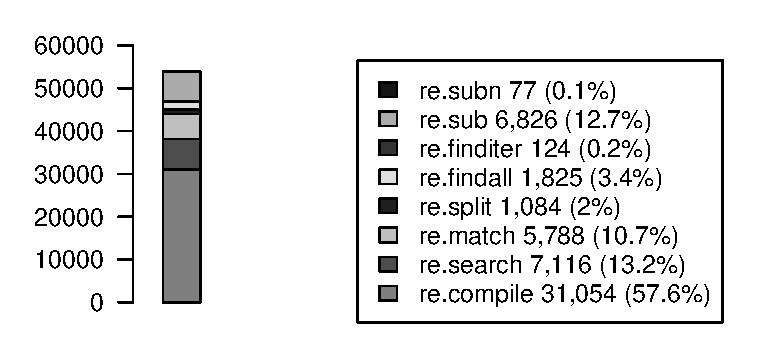
\includegraphics[width=\columnwidth]{../analysis_output/partFunctions.eps}
\caption{How often are the 8 re functions used?}
\label{fig:partFunctions}
\end{figure}

As seen in Figure~\ref{fig:partFunctions} The `compile' function encompasses \DTLfetch{data}{key}{percentCompile}{value}\% of all usages, even though every compiled regex object can only be used by calling other functions.  (TODO-Why?)

\begin{figure}[htb]
\centering
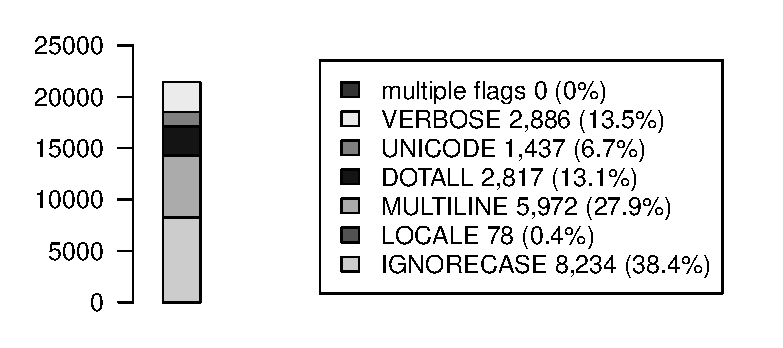
\includegraphics[width=\columnwidth]{../analysis_output/partFlags.eps}
\caption{Which behavioral flags are used?}
\label{fig:digraph}
\end{figure}

\DTLfetch{data}{key}{percentFlags0}{value}\% of all regex usages did not use a flag or specified a non-behavioral flag (default or debug).  Of all behavioral flags used, ignorecase (\DTLfetch{data}{key}{percentI}{value}\%) and multiline (\DTLfetch{data}{key}{percentM}{value}\%) were the most frequently used.  It is also worth noting that although multiple flags can be combined using a bitwise or, this was never observed. (remove this last part if it is observed later)

\subsubsection{\centerline{GENERAL CHARACTERISTICS OF REGEXES FOUND}}

...TODO

\subsubsection{\centerline{Top 10 Regex Patterns by weight}}


\begin{table}
\caption{ \label{}}
\begin{center}
\begin{tabular}{lc}
\toprule
pattern & weight \\ 
\midrule
\begin{minipage}{2.3in}
\begin{verbatim}
'\\s+'\end{verbatim}
\end{minipage}
& 181 \\ 
\midrule
\begin{minipage}{2.3in}
\begin{verbatim}
'\\s'\end{verbatim}
\end{minipage}
& 78 \\ 
\midrule
\begin{minipage}{2.3in}
\begin{verbatim}
'\\d+'\end{verbatim}
\end{minipage}
& 70 \\ 
\midrule
\begin{minipage}{2.3in}
\begin{verbatim}
'[\\x80-\\xff]'\end{verbatim}
\end{minipage}
& 69 \\ 
\midrule
\begin{minipage}{2.3in}
\begin{verbatim}
'\nmd5_data = {\n([^}]+)}'\end{verbatim}
\end{minipage}
& 69 \\ 
\midrule
\begin{minipage}{2.3in}
\begin{verbatim}
'\\\\(.)'\end{verbatim}
\end{minipage}
& 67 \\ 
\midrule
\begin{minipage}{2.3in}
\begin{verbatim}
'([\\\\"]|[^\\ -~])'\end{verbatim}
\end{minipage}
& 66 \\ 
\midrule
\begin{minipage}{2.3in}
\begin{verbatim}
'(-?(?:0|[1-9]\\d*))(\\.\\d+)?([eE][-+]?\\d+)?'\end{verbatim}
\end{minipage}
& 61 \\ 
\midrule
\begin{minipage}{2.3in}
\begin{verbatim}
'[^]]+?\\] +([0-9.]+): (\\w+) <-(\\w+)'\end{verbatim}
\end{minipage}
& 60 \\ 
\midrule
\begin{minipage}{2.3in}
\begin{verbatim}
'.*rlen=([0-9]+)'\end{verbatim}
\end{minipage}
& 57 \\ 
\bottomrule
\end{tabular}
\end{center}
\end{table}


%\DTLfetch{topNW}{key}{1}{pattern}
